\chapter{Конструкторская часть}
\label{cha:design}

В данной части будут приведены схемы алгоритмов Левенштейна в рекурсивной и матричной реализации и Дамерау-Левенштейна.

\section{Разработка алгоритмов}
% сюда схемы алгоритмов

Далее указаны разработанные схемы алгоритмов Левенштейна и Дамерау-Левенштейна.
Будем считать, что известны следующие функции:
определения длины строки,
поиска максимума и минимума среди нескольких чисел.
Для матричных реализаций требуется наличие функции, динамически выделяющей память.


\begin{figure}
    \centering
    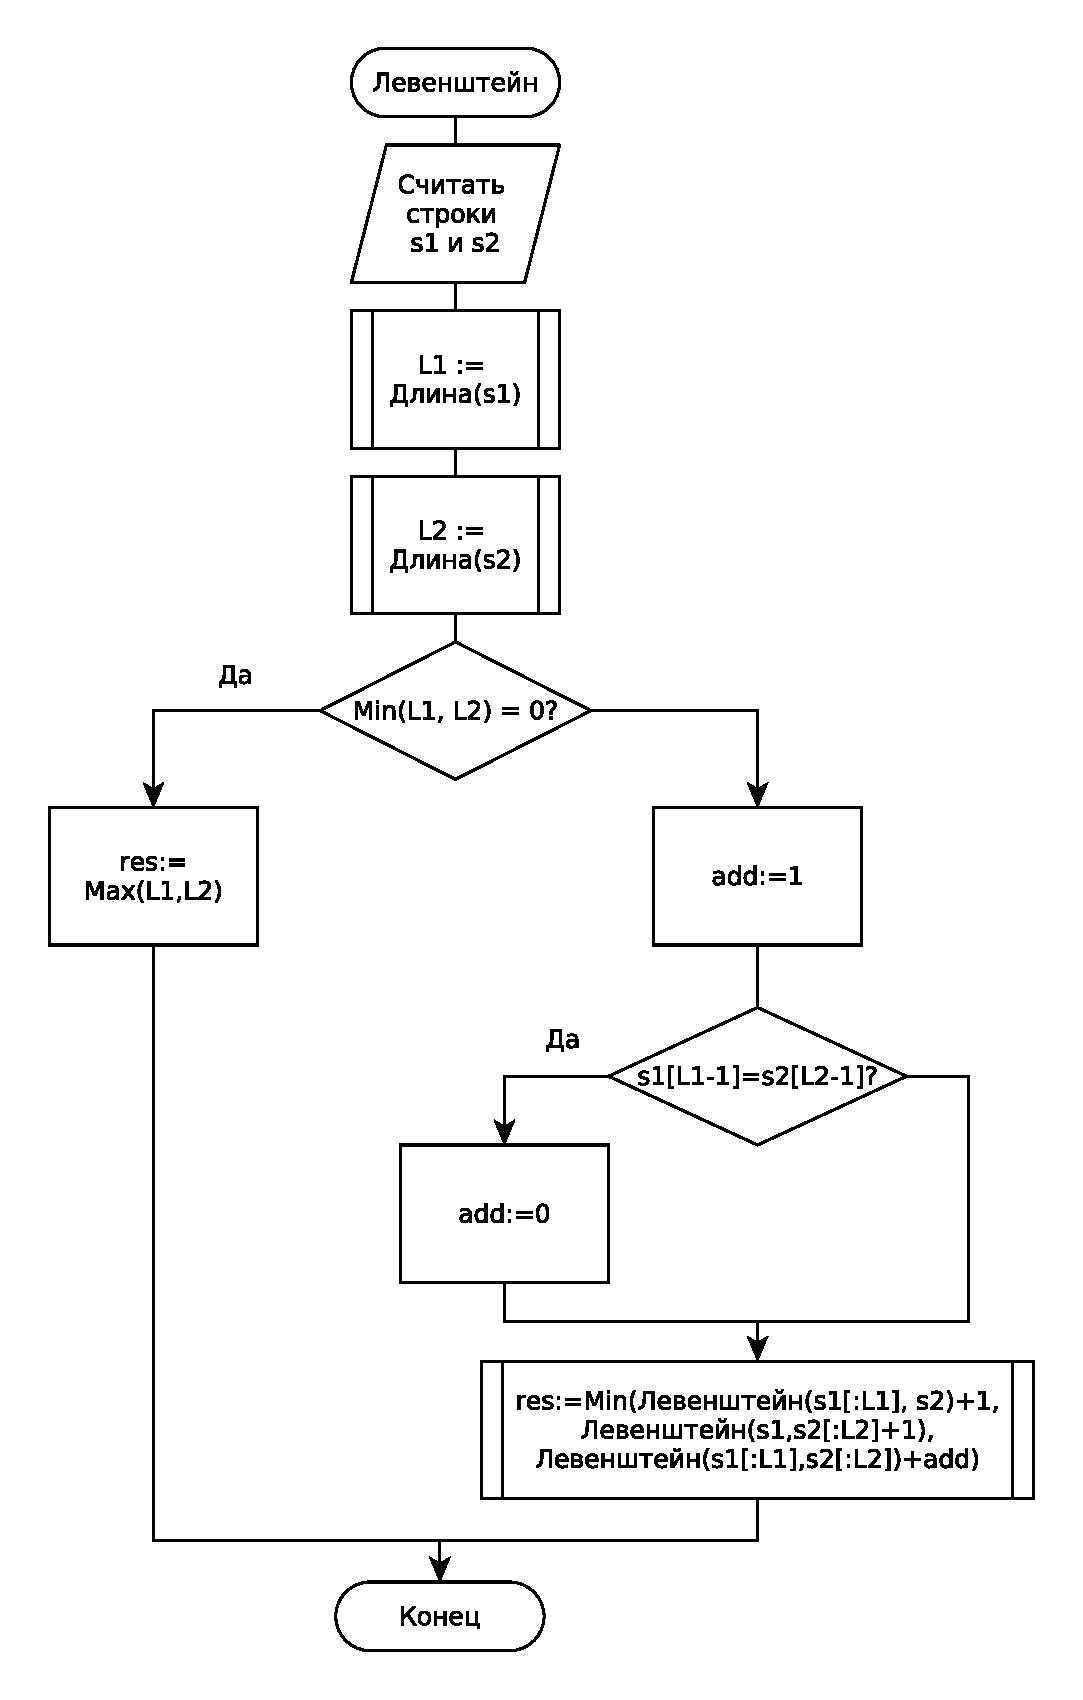
\includegraphics[height=0.9\textheight]{schemes/levenshtein-recursive-eps}
    \caption{Схема рекурсивного алгоритма Левенштейна}
    \label{levenshtein-recursive-scheme}
\end{figure}

\begin{figure}
    \centering
    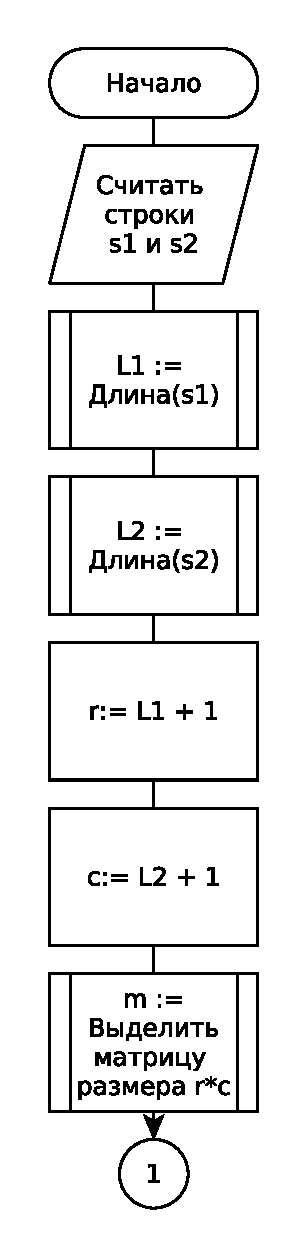
\includegraphics[height=0.9\textheight]{schemes/levenshtein-iterative-eps-1}
    \caption{Схема матричного алгоритма Левенштейна. Часть 1.}
    \label{levenshtein-iterative-scheme-part-1}
\end{figure}

\begin{figure}
    \centering
    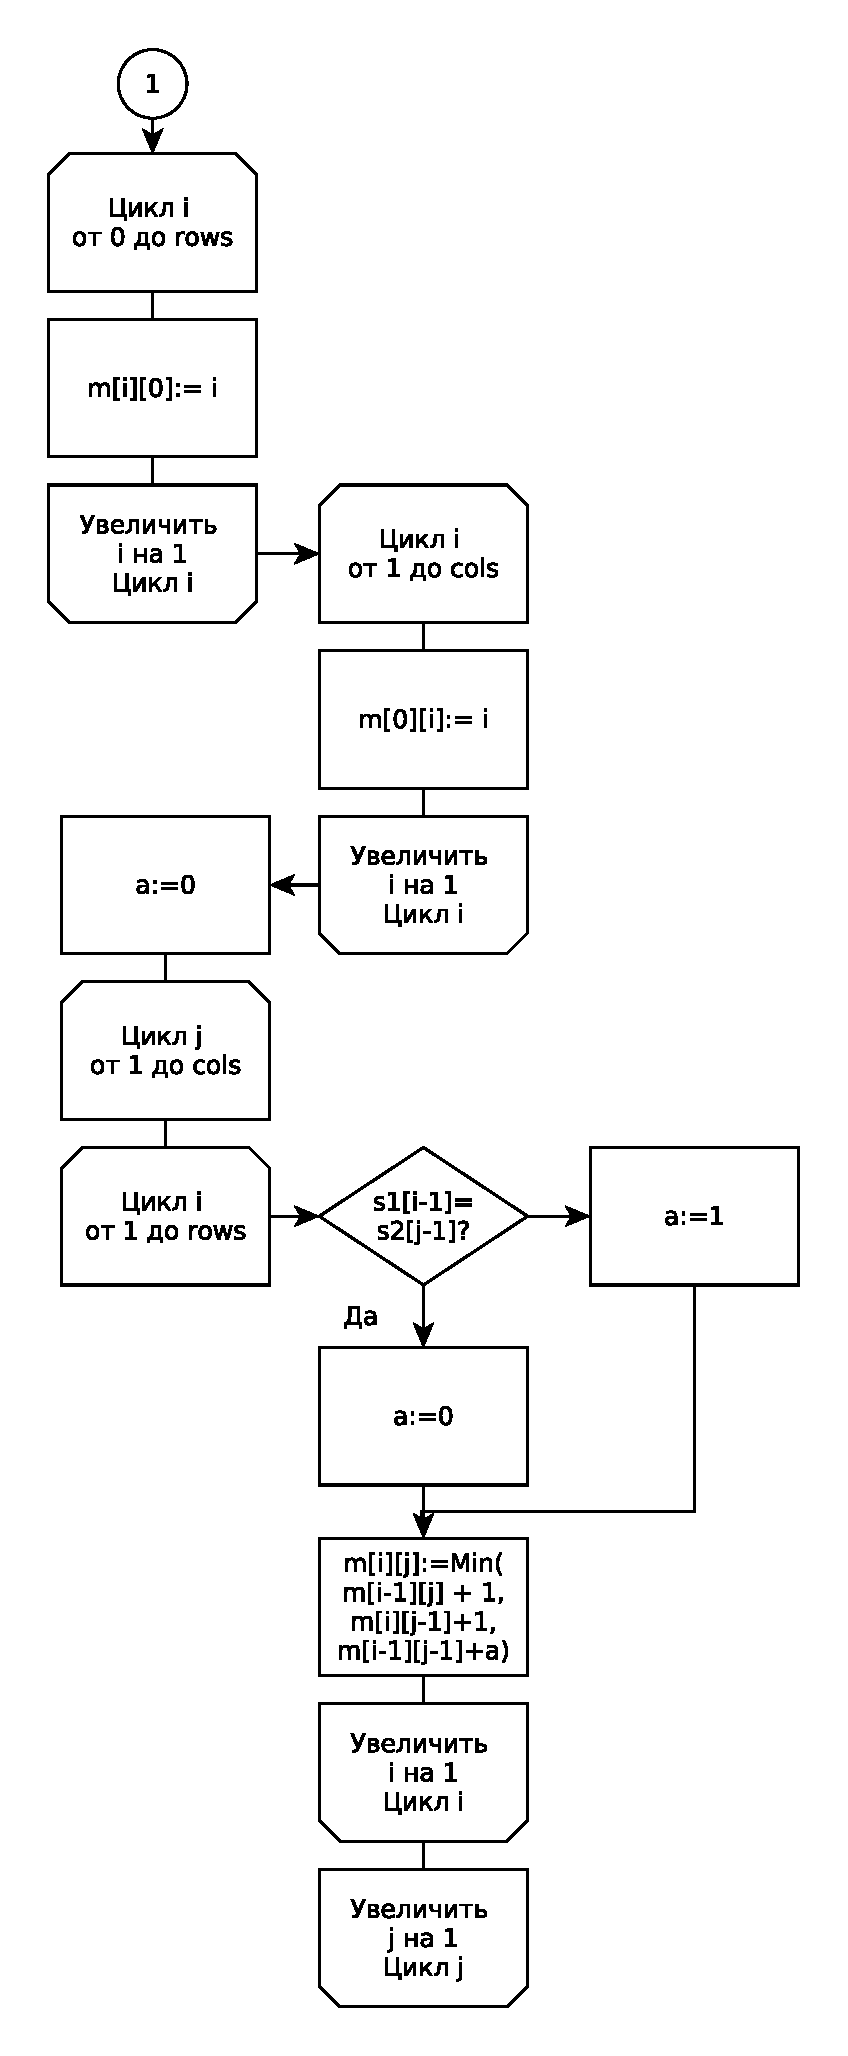
\includegraphics[height=0.9\textheight]{schemes/levenshtein-iterative-eps-2}
    \caption{Схема матричного алгоритма Левенштейна. Часть 2.}
    \label{levenshtein-iterative-scheme-part-2}
\end{figure}

\begin{figure}
    \centering
    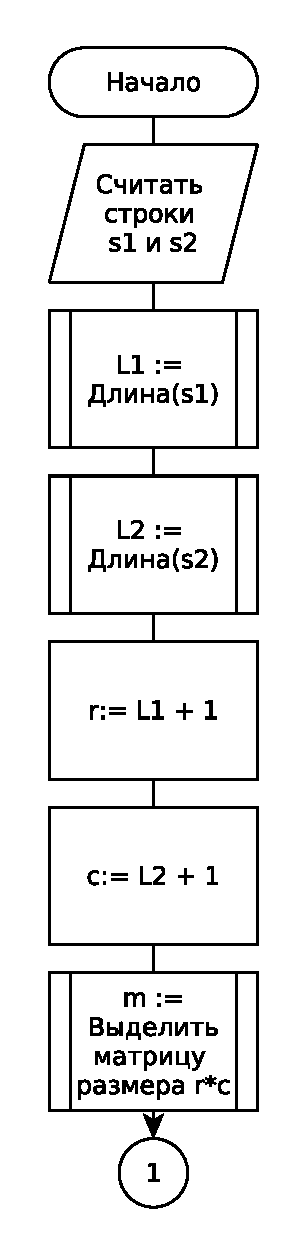
\includegraphics[height=0.9\textheight]{schemes/levenshtein-damerau-eps-1}
    \caption{Схема алгоритма Дамерау-Левенштейна. Часть 1.}
    \label{levenshtein-damerau-scheme-part-1}
\end{figure}

\begin{figure}
    \centering
    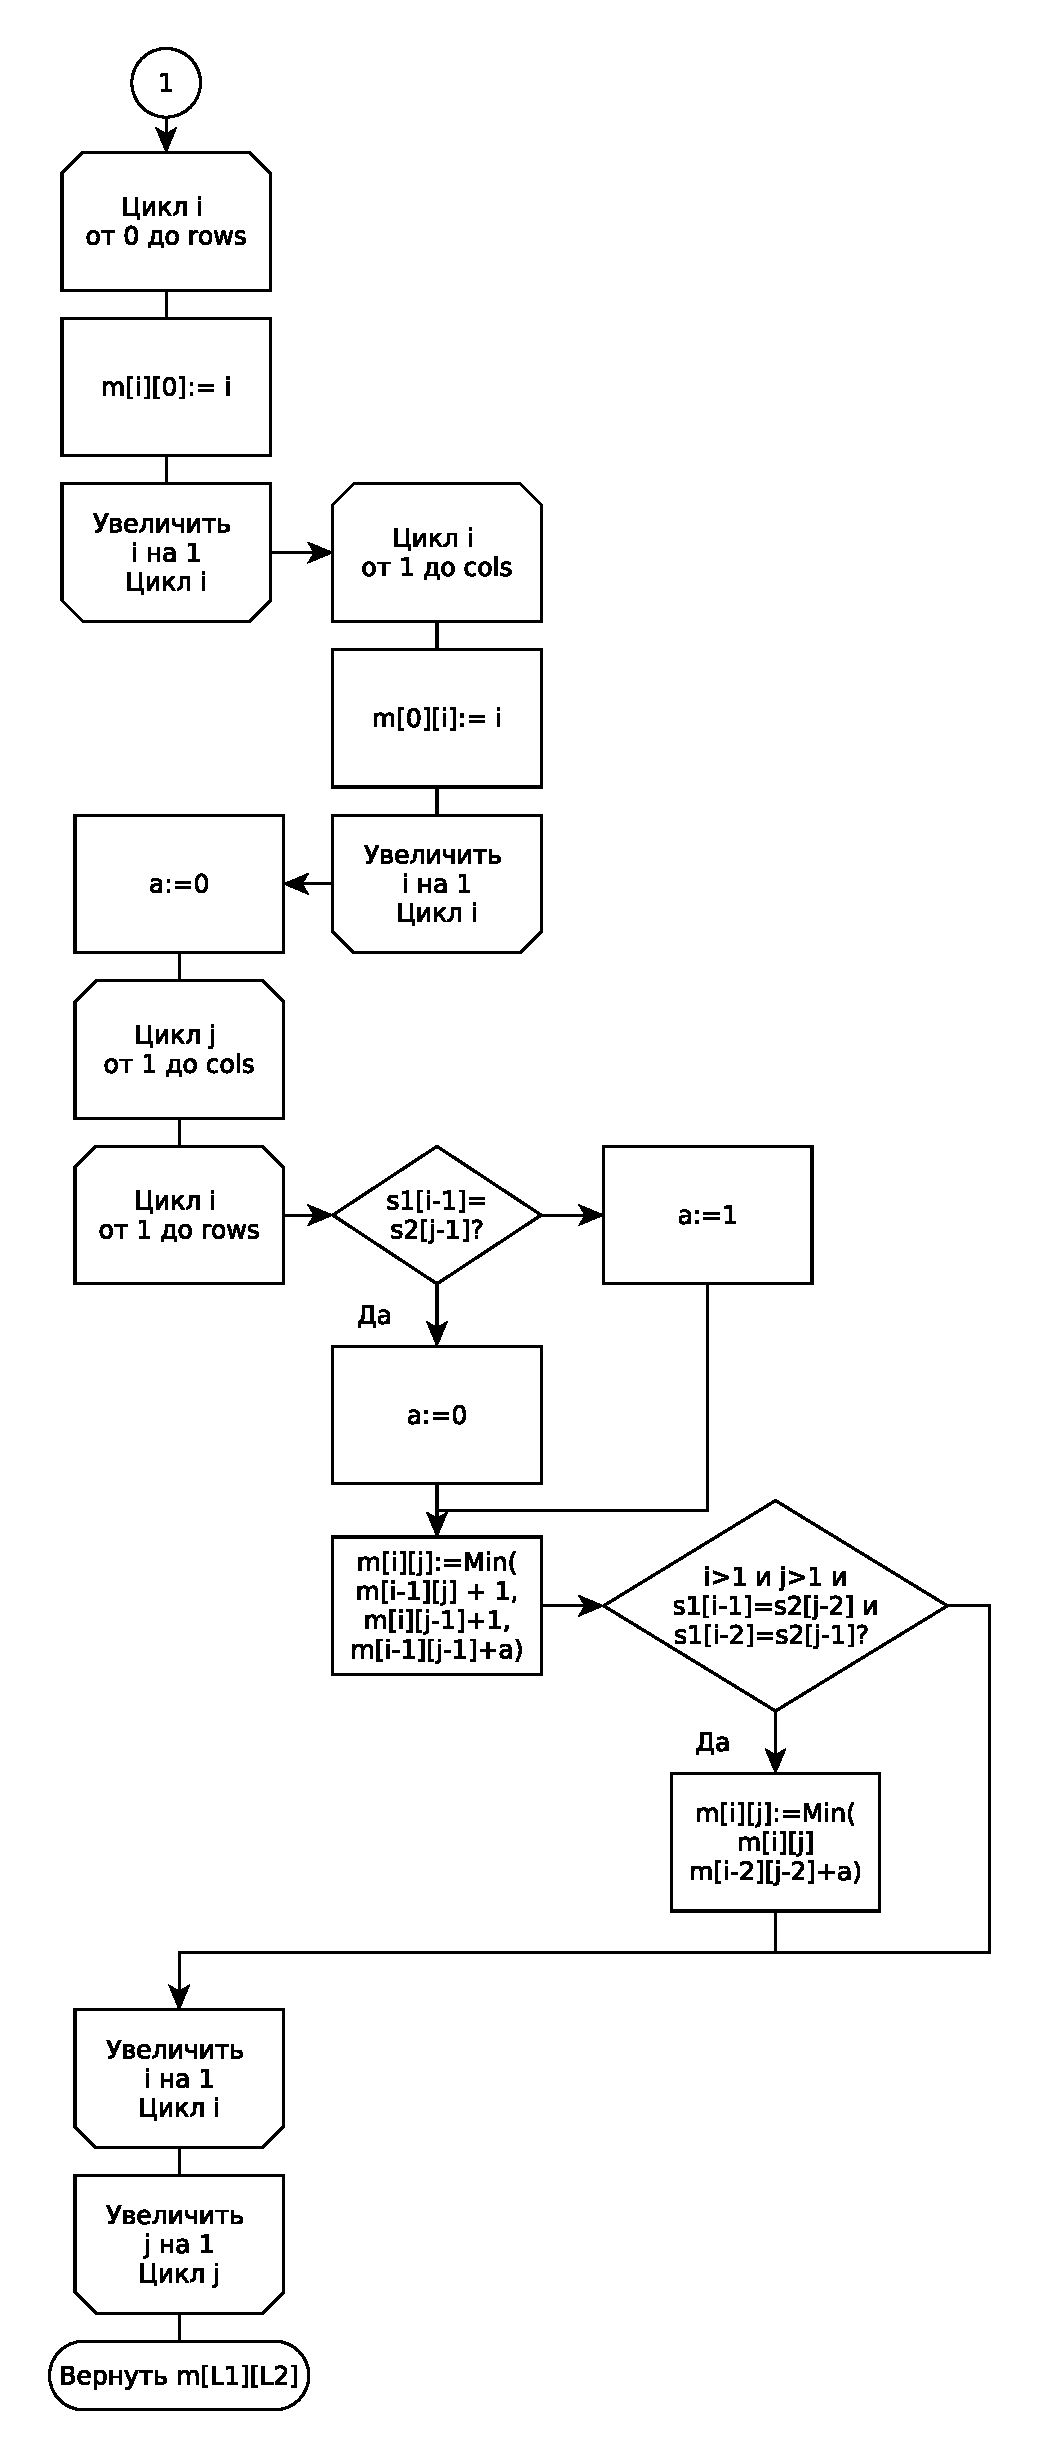
\includegraphics[height=0.9\textheight]{schemes/levenshtein-damerau-eps-2}
    \caption{Схема алгоритма Дамерау-Левенштейна. Часть 2.}
    \label{levenshtein-damerau-scheme-part-2}
\end{figure}

\FloatBarrier

\section{Сравнительный анализ рекурсивной и нерекурсивной\\ реализаций}

Какой-то текст
